\documentclass[10pt]{article}
\usepackage[margin=1.05in]{geometry}
\usepackage{amsmath, amssymb, amsthm}
\usepackage{graphicx}
\usepackage{xcolor}
\usepackage[colorlinks=true, linkcolor=blue, citecolor=blue]{hyperref}
\graphicspath{{figs/}}

\theoremstyle{definition}
\newtheorem{definition}{Definition}
\newtheorem{example}{Example}

\title{Compositionality: hierarchy, and the pressures for breadth and depth}
\author{Asvin G.\thanks{Draft; experiments and analysis joint with Claude. Code: \texttt{github.com/asving/RRXOR}, \texttt{correction\_geometry/}.}}
\date{Draft of \today}

\begin{document}
\maketitle

\section{What is compositionality?}

There is a generally shared intuition that the ability to compose outputs, behaviours or functions is a powerful technique to create more capable systems, and there has been a fair amount of work studying how compositional LLMs are at a behavioral level. However, there is a puzzle in applying this lens to the internal circuitry of a neural network. A deep network is, by definition, a composition of functions and so automatically compositional under our above definition.

However, there is a clear difference between different networks in how compositional they seem to our intuition (as we will see in examples below). I will argue that what we really want (as suggested by Danaja) is that the network solves a task family by combining a few \textbf{computational units} (i.e., functions or subcircuits part of the computational graph of the trained network), each useful across many tasks --- so that when a new task arrives, the expressivity \emph{reachable in a short period of training} is much higher than raw parameter count suggests. This ties the decomposition of the circuit to the structure of the task, and therefore makes the decomposition not automatic.

Before going further we fix the basic objects.

\begin{definition}[network, parameters]
A neural architecture defines a differentiable map $f(x;\theta)$ from inputs to output logits, where $\theta \in \mathbb{R}^P$ is the concatenation of all trainable weights. Training is stochastic gradient descent on $L(\theta) = \mathbb{E}_x\, \ell(x;\theta)$ for a per-example loss $\ell$ (cross-entropy for the sequence tasks; one regression experiment in section~2 uses squared loss). Whenever we write a gradient below, it is a vector in $\mathbb{R}^P$, taken with respect to this $\theta$ at the current training point $\theta_t$.
\end{definition}

\begin{definition}[circuit]\label{def:circuit}
The computation of $f(\cdot;\theta)$ unrolls into a directed acyclic computational graph whose nodes are intermediate quantities (neurons, attention scores, residual-stream coordinates at a given layer and position) and whose edges carry the weight entries that connect them. A \emph{circuit} $C$ is a subgraph together with the designation of its edge weights as free: the circuit's tangent space is the coordinate subspace of $\mathbb{R}^P$ spanned by $C$'s free weights, and $P_C$ denotes the coordinate projection onto it (so $P_C\, g$ is simply the gradient restricted to $C$'s weights). In practice we rarely attribute individual weights to circuits; instead we measure a circuit through an \emph{interface} at a chosen site, a construction Definition~\ref{def:interface} makes precise and which agrees with the subgraph view when the subgraph is the one feeding the interface.
\end{definition}

\begin{definition}[breadth and depth]
The \textbf{breadth} of a circuit is the number of distinct computational units that feed into it, and its \textbf{depth} is the number of computational units it serially consumes before reaching the input.
\end{definition}

Examples will make clear how we are using these terms; in this draft they are organizing vocabulary rather than measured quantities. We first explain a possible incentive for neural networks to learn compositionally broad circuits, coming directly from the number of distinct `tasks' the network needs to solve.

\section{Breadth: the pressure to share across tasks}

The simplest setting is when each circuit is the solution to a particular task in our task family. For instance, in a next-token prediction task on a sequence generated by an HMM, the tasks might be indexed by the hidden state of the system (or some coarsening of such). The network then has to learn a different solution conditional on the hidden state, learn to estimate its belief distribution over these hidden states, and use this distribution to combine the different solutions. Let us first investigate the potential learning pressures in this simple compositional circuit. Our two running examples realize the two natural shapes of such a task family: tasks indexed by a hidden \emph{state} (Example~\ref{ex:rrxor}) and tasks indexed by a \emph{composition} of active subprocesses (Example~\ref{ex:comp}). A note on vocabulary: Definition~3 defined breadth as the fan-in of a circuit, while the pressure studied here acts on the units themselves, through how many tasks consume each one. The two meet in the claim this section argues: circuits of high fan-in get built \emph{because} their parts are widely consumed.

\begin{example}[RRXOR]\label{ex:rrxor}
An example to keep in mind throughout is the RRXOR sequence, of the form $\ldots\{\text{random bit}\}\{\text{random bit}\}\{\text{xor of the previous two}\}\ldots$ Precisely: draw iid fair bits $r_1^{(k)}, r_2^{(k)}$ and form blocks $B^{(k)} = (r_1^{(k)}, r_2^{(k)}, r_1^{(k)} \oplus r_2^{(k)})$; concatenate the blocks and emit a window of length $L$ starting at a uniformly random offset $o \in \{0,1,2\}$. Each position $t$ then carries a hidden phase $p_t = (o+t) \bmod 3$: positions with $p_t \in \{0,1\}$ are free bits, and $x_t = x_{t-1} \oplus x_{t-2}$ whenever $p_t = 2$:
$$\underbrace{1 \quad 0 \quad \mathbf{1}}_{r_1\ \ r_2\ \ \oplus} \qquad \underbrace{1 \quad 1 \quad \mathbf{0}}_{r_1\ \ r_2\ \ \oplus} \qquad \underbrace{0 \quad 1 \quad \mathbf{1}}_{r_1\ \ r_2\ \ \oplus} \qquad (\text{bold} = \text{determined; a window may begin mid-block}).$$ One way to classify the tasks is as `predicting a random bit' and `predicting the xor of the previous two bits'; which prediction applies is indexed by a belief over the current phase. The generator's minimal causal machine has 5 states (nothing pending / one pending bit $\times 2$ / pending xor $\times 2$). An observer ignorant of $o$ must synchronize: its belief state is the posterior over phase together with the last two bits, and exact enumeration of this filter gives 51 reachable states which minimize to exactly \textbf{36} under bisimulation, i.e.\ keeping only information relevant for predicting the future. The Bayes floor is $\ln 2$ at free positions and $0$ at xor positions once synchronized. (The three state counts are needed only in section~4.2.)
\end{example}

Each `solution' receives positive gradient pressure on the tokens corresponding to its hidden states. On other hidden states, we might simplify the analysis by assuming that the gradient pressure is a random vector, and expect that the sum of the gradient contribution over all the other hidden states cancels out relative to the positive gradient pressure.

From this perspective, any circuit in the network receives a mean gradient relative to each task, and the total amplification it receives depends on the total gradient vector across all tasks. This will be large if there are many tasks with an `aligned' mean-gradient vector, i.e., the way the circuit is used across different tasks is roughly identical. On the contrary, the total contribution will be $\approx 0$ if the circuit is used in a different way in each task.

\begin{definition}[gradient vectors]\label{def:grads}
For a task $\tau$ with data distribution $D_\tau$ and per-example loss $\ell_\tau(x;\theta)$, distinguish three objects:
$$\underbrace{\nabla_\theta\, \ell_\tau(x;\theta)}_{\text{per-example (random)}}, \qquad
\underbrace{g_\tau(\theta) = \mathbb{E}_{x\sim D_\tau}\!\left[\nabla_\theta\, \ell_\tau(x;\theta)\right]}_{\text{task gradient (the drift)}}, \qquad
\underbrace{\hat g^{(B)}_\tau}_{\text{batch: drift} \,+\, \text{noise of covariance } \Sigma_\tau/B}.$$
In the HMM setting the tasks share one next-token loss and differ only in conditioning: $D_\tau$ is the distribution of contexts given hidden state $\tau$, so $g_\tau$ is the state-conditional mean gradient.
\end{definition}

\begin{definition}[alignment and drive]\label{def:align}
For a circuit $C$ with projection $P_C$ (Definition~\ref{def:circuit}), the alignment of two tasks on $C$ and the aggregate drive on $C$ are
$$\mathrm{align}(\tau,\tau' \mid C) = \frac{\langle P_C\, g_\tau,\, P_C\, g_{\tau'}\rangle}{\|P_C\, g_\tau\|\, \|P_C\, g_{\tau'}\|},
\qquad
\mathrm{drive}(C) = \Big\| \sum_\tau w_\tau\, P_C\, g_\tau \Big\|^2,$$
where $w_\tau$ is the fraction of tokens that both carry loss and belong to task $\tau$ (in the HMM setting: the fraction of positions whose hidden state is $\tau$). With $n$ aligned \emph{consumers} (tasks whose loss gradient reaches the circuit) the drive grows like $n^2$; with unaligned (randomly oriented) consumers like $n$, no better than noise; with sign-opposed consumers it can vanish at positive per-task norms. For a single consumer, drive is proportional to its weight, which is how the empirical `drive law' $\tau_{\text{learn}} \propto 1/\varphi$ of Figure~\ref{fig:b3} (experiment B3 below) follows: the use frequency $\varphi$ is exactly $w_\tau$.
\end{definition}

\paragraph{The financing picture.} We think of the circuits as being 'bought' through tokens, and use economic vocabulary to emphasize this perspective throughout. A circuit is \emph{financed} when it receives coherent aggregate drive (Definition~\ref{def:align}); several consumers \emph{co-finance} a shared circuit when their task gradients align on it, which is what makes the drive grow quadratically rather than linearly in their number. Demand for a variable is \emph{manufactured} when an upstream circuit's formation creates coherent drive where there was none, and is \emph{destroyed by satisfaction} once the variable is supplied and the correction it carried vanishes (both measured directly in Figure~\ref{fig:demand}, left). Co-financing \emph{decoheres} when the consumers stop agreeing on how the shared circuit should be used, collapsing the aggregate drive at constant per-consumer magnitudes (Figure~\ref{fig:demand}, right). The budget is gradient coherence; the price of a circuit is the inverse of its accessibility (section~\ref{sec:ease}).

\begin{example}[factored composition]\label{ex:comp}
Our second running example. Four independent hidden-Markov factors (small 3-state processes) share one output alphabet; each sequence draws a \emph{mask}, one of the $2^4 - 1 = 15$ nonempty subsets of factors, held fixed for the sequence. At each step, with probability $\epsilon$, the factors active under the mask emit \emph{jointly} (copying a designated leader factor) rather than independently, so the mask is both inferable from the sequence and predictively relevant: the coupling is the only footprint of composition. The tasks of Definition~\ref{def:grads} are the masks. A model trains on 10 masks with the remaining 5 held out, and the \emph{composition score} on held-out masks is $(\mathrm{CE}_{\text{restricted}} - \mathrm{CE}_{\text{model}})/(\mathrm{CE}_{\text{restricted}} - \mathrm{CE}_{\text{oracle}})$, where $\mathrm{CE}_{\text{model}}$ is the trained network's cross-entropy on held-out-mask sequences. Read it as: $1$ = the model predicts as if the new composition were already in its repertoire (construction from parts); $0$ = no better than optimal reuse of stored compositions; negative = committing to a wrong stored composition harder than optimal reuse would. The two references are instances of one machine. For a hypothesis set $H \subseteq \mathcal{C}$ of masks, let $p_H$ be the exact Bayes filter that maintains the joint posterior over the mask and the factors' hidden states,
$$b_t(c, s) \;\propto\; \pi(c)\, \Pr\!\left(x_{1:t},\, s \mid c\right) \cdot \mathbf{1}[c \in H], \qquad p_H(x_{t+1} \mid x_{1:t}) = \sum_{c \in H,\, s} b_t(c, s)\, \Pr(x_{t+1} \mid c, s),$$
with $\pi$ uniform on $H$ and $s$ ranging over the joint hidden states of the four factors under the coupled emission model. Then $\mathrm{CE}_{\text{oracle}}$ is the cross-entropy of $p_{\mathcal{C}}$ (all 15 masks) and $\mathrm{CE}_{\text{restricted}}$ that of $p_{\mathcal{C}_{\text{train}}}$ (the 10 training masks), both evaluated on held-out-mask sequences. The restricted machine thus knows the factors and the coupling perfectly and infers optimally, but can only interpret the sequence as one of the compositions it has seen: it is the \emph{best possible reuse strategy}, and the score is the fraction realized of the benefit of extending the hypothesis space from seen to novel combinations. The natural candidate units are the four per-factor predictors plus a \emph{binding} stage that combines the active ones; the formation, reuse, and erosion of exactly this decomposition is what B1 (Figure~\ref{fig:b1}) and the decoherence analysis (Figure~\ref{fig:demand}, right) trace.
\end{example}

These three regimes are exactly the ones realized by the experiments below: single-consumer drive setting formation speed (B3), aligned co-financing and its erosion (B1), and sign-opposed conflict (B2). Each experiment is summarized by one figure; the text records only the task and how the figure was obtained.

\paragraph{B1: compositional solutions are found first, and can erode.}
Task: the factored composition of Example~\ref{ex:comp}, learned by a small transformer (4 layers, $d = 128$, $0.8$M parameters). Figure~\ref{fig:b1} plots the held-out composition score against training step (logged every 100 steps; one run per coupling strength $\epsilon$). The compositional solution appears early in both regimes and remains partial (plateau $\approx 0.7$ even when stable). The plateau is worth pausing on: held-out behavior carries zero training weight, so the general binding rule and a bundle of mask-specific solutions are equally good on the training loss, and the score records which of these training-equivalent solutions selection favors. Ten masks co-financing shared machinery is what pushes the score well above zero; nothing pushes it to one. Probes confirm the parts are not the problem: per-factor representations generalize at $R^2 \approx 0.9$--$1.0$ on held-out masks, and the shortfall is in the binding. Under approximate coupling the partial solution additionally erodes as an in-distribution-specialized solution takes over (the aligned demand of the training masks decoheres; see section~\ref{sec:ease}).

\begin{figure}[t]\centering
\includegraphics[width=0.5\linewidth]{b1_transience}
\caption{Held-out composition score (Example~\ref{ex:comp}) over training, one run per condition. Approximate coupling ($\epsilon=0.8$): early peak, then erosion. Exact coupling ($\epsilon=1.0$): stable and still improving. The solution that replaces the eroding compositional one is more accurate on the \emph{training} masks only; its held-out score is what decays.}\label{fig:b1}
\end{figure}

\paragraph{B2: misaligned gradients are absorbed by splitting.}
Task (the \emph{sign exercise}): two scalar regression targets computed from a shared latent $z$, $t_A = \mathrm{relu}(z)$ and $t_B = (1-\lambda)\,\mathrm{relu}(z) + \lambda\,\mathrm{relu}(-z)$, learned by a small ReLU network (8 hidden units) with one shared feature layer, so the dial $\lambda$ moves the two tasks from identical to opposite-sign use of the same latent. Figure~\ref{fig:b2} plots three quantities against $\lambda$ (means over 4 seeds; heterogeneous units share the axis): the realized alignment $\mathrm{align}(A,B\mid C)$ with $P_C$ the restriction to the shared layer's weights; the normalized error of a network \emph{forced} to route both tasks through a single shared unit; and the Jaccard overlap between the unit sets each task relies on (by per-unit ablation) in an unconstrained network. As alignment crosses to negative, the forced-shared solution degrades while the free network keeps zero error by \emph{reducing} unit sharing ($.73 \to .41$): misaligned demand is absorbed by partial duplication.

\begin{figure}[t]\centering
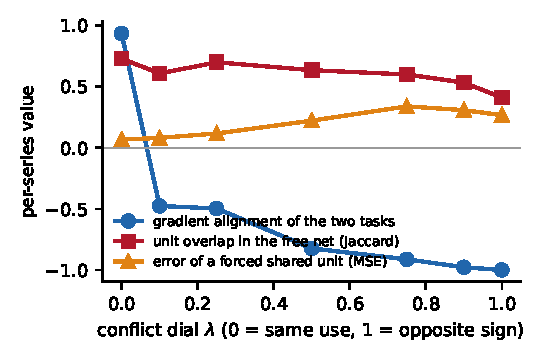
\includegraphics[width=0.5\linewidth]{b2_conflict}
\caption{The sign exercise: sweeping the conflict dial $\lambda$ from coherent to sign-opposed use of a shared feature. Series are 4-seed means; units differ per series (alignment is a cosine in $[-1,1]$, overlap is a Jaccard index in $[0,1]$, forced-share error is a normalized MSE).}\label{fig:b2}
\end{figure}

\paragraph{B3: more-used circuits form first, and are chosen.}
Two measurements. Left of Figure~\ref{fig:b3}: a gated composite task where a subcircuit's inputs are informative on a fraction $\varphi$ of examples (the use frequency); we log the step at which the subcircuit's accuracy on its own targets crosses $0.9$, across $\varphi \in \{1.0, 0.3, 0.1, 0.03\}$ (points are 2-seed means). Formation time follows $\tau \propto 1/\varphi$: drive sets speed. Right: a task presents the same information in two behaviorally equivalent views, one shared across $T$ tasks and one private. Reliance on a view is the normalized accuracy drop when that view is ablated; we plot the difference (shared $-$ private) against $T$, alongside the symmetric control in which both views are shared. A second control, forcing the private view, confirms the private route is fully learnable; it is not plotted. The network increasingly routes through the shared view as its reuse grows.

\begin{figure}[t]\centering
\includegraphics[width=0.78\linewidth]{b3_drive}
\caption{Left: the drive law, formation time vs.\ use frequency. Right: reuse-scaled selection between equivalent circuits.}\label{fig:b3}
\end{figure}

Supporting evidence: across $\sim$140 networks in two task families, modularity (measured as held-out transfer of the learned pairwise gates) correlates with evolvability (behavioral change per unit of small weight perturbation) at matched loss (Spearman $0.65$--$0.73$).

\section{Depth: the pressure to consume other units}

We now explain a possible incentive for neural networks to learn compositionally deep circuits. At the same time, this also offers an explanation for why networks with a residual stream represent information linearly (explained to me by Francesco). The basic idea is that information that is consumed by many downstream circuits is best represented linearly: the attention and MLP operators add to the residual stream, but with a norm that is relatively small compared to the residual vector in the typical case. Therefore information represented linearly can persist for many layers in a relatively stable format.

The main obstacle for a transformer network is integrating information across many token positions, i.e., computing joint correlation functions in many variables. The difficulty rises with the number of variables because the \emph{drift self-cancels}: for a genuinely joint function of $k$ inputs (a parity is the extreme case), flipping any one input flips the target, so per-example gradients cancel in matched pairs and the population gradient $g_\tau$ survives only through higher-order couplings in the weights. The per-example gradients are not small; they point in data-dependent directions that average away. Figure~\ref{fig:degree} shows this measured directly: we trained a 1-layer transformer on three single-route tasks whose answers are functions of 1, 2, and 3 source tokens respectively (a lookup, an xor, a 3-parity; two seeds each), recorded the time $\tau_{95}$ to $95\%$ held-out accuracy, and separately measured at initialization the drift-to-noise ratio $\mathrm{SNR} = \|\mathbb{E}\nabla_\theta m\|^2 / \mathbb{E}\|\nabla_\theta m\|^2$ --- the fraction of the gradient's power that is systematic --- of the answer margin $m$, the correct-answer logit minus the wrong-answer logit (Definition~\ref{def:gdisc} makes both precise; expectations estimated from $2{,}560$ examples at the same initialization for all three tasks). Small open markers in Figure~\ref{fig:degree} are the individual seeds. Learning time multiplies by ${\sim}4$ per added variable while $\tau \cdot \mathrm{SNR}$ stays constant to within a factor of $2$. On tree-structured tasks (latent hierarchies in which each level generates the next through a fixed noisy channel; studied in the companion repository) the attenuation has a closed form: crossing one latent level multiplies the usable squared correlation by that level's strong-data-processing (SDPI) constant $\eta_\ell = \lambda_2(T_\ell)^2$, the squared second singular value of the level's channel --- the fraction of squared correlation that survives the crossing --- giving a geometric ladder of learning times.

\begin{figure}[t]\centering
\includegraphics[width=0.45\linewidth]{degree_ladder}
\caption{Why higher-order correlations are harder: time-to-learn against the inverse drift-to-noise ratio of the circuit's teaching signal at initialization, for circuits of input degree 1/2/3 on one architecture. The line is $\tau = c/\mathrm{SNR}$ with a single shared constant.}\label{fig:degree}
\end{figure}

However, when the token stream is such that some tasks are easy and depend on, say, the current token and previous token, and in computing this easy solution the network writes some information to an intermediate layer that can then be combined with a previous token to solve harder tasks, we will see precisely a compositionally deep circuit emerging.

\begin{figure}[t]\centering
\includegraphics[width=0.48\linewidth]{rrxor_formation}\hfill
\includegraphics[width=0.5\linewidth]{m27_cascade}
\caption{Left: RRXOR formation; per-class CE (top) and probability of outputting the xor of the previous two bits (bottom); the two free-bit classes nearly coincide throughout, as symmetry demands. Colors are assigned per panel, and the two columns use different time axes (the runs differ $4\times$ in length). Right: the matryoshka cascade (period-27 exception tower over the xor rule: XNOR at two of nine blocks, one block flipping back); the exception classes' CE \emph{spikes} exactly while the model's probability of outputting plain xor on them \emph{rises}: the net confidently bets the wrong rule until the correction that distinguishes the blocks is financed by those very errors.}\label{fig:rrxor}
\end{figure}

RRXOR is the minimal case of this. The xor function is a two-position circuit, directly financed at every third position (coherent drive arrives for it from step 0), and it forms almost immediately. Once it exists, its \emph{violations} become a new intermediate variable that localizes the phase: the teaching signal for the phase circuit literally does not exist until the xor unit computes. Figure~\ref{fig:rrxor} shows the formation: from 79 checkpoints of a single 4-layer next-token run we plot, per position class, the cross-entropy and the probability mass the model assigns to the xor of the previous two bits. The xor circuit forms first and is applied at the right positions only as the phase circuit sharpens.



The same structure iterated at nested scales is the matryoshka cascade (Figure~\ref{fig:rrxor}, right). The process extends RRXOR to period 27: a super-period of nine consecutive $(r_1, r_2, \text{det})$ blocks in which the deterministic slot obeys $\text{det} = r_1 \oplus r_2 \oplus \text{rule}(b)$, The rule is $1$ (XNOR) on blocks $b \in \{2, 5\}$ and $0$ elsewhere. Block $8$ is tracked as its own class (`flip'): it is the position where the mod-9 pattern would suggest a third exception, but the rule flips back to plain xor. Windows start at a random offset mod 27, so all block identities must be inferred from content. The plot is generated from the training log of one 6-layer run: per class, the CE and the probability assigned to plain xor. The manufactured-gradient signature is the rise of the wrong bet: the model's probability of answering plain xor on the XNOR class \emph{rises above chance} while that class's CE spikes, and those errors are what finance the block-classification circuit that then resolves both. A family of tree-structured grammar tasks (studied in the companion repository) generalizes this quantitatively: learning time per level multiplies by the inverse SDPI constant of the level crossed.

Note that the story we are telling here is not necessarily a hard constraint. First, depth-by-bootstrapping is primarily about \emph{speed and staging, never possibility} at our scales: it is a story about sample efficiency, as our experiments illustrate. Second, sharp stage boundaries require \emph{gating} (the later gradient not existing until the earlier circuit forms, as in RRXOR and the matryoshka tower); mere complexity separation gives ordered but overlapping onsets.

\section{Compositionality is a learning-dynamics notion}\label{sec:ease}

The upshot of the previous two sections is that breadth and depth are selected by the same currency: coherent gradient drive. This makes compositionality a learning-dynamics notion rather than an expressivity notion. The expressivity that matters is the set of functions reachable in a short window of SGD from the current parameters; computational units are what make this set large, because aligned consumers accumulate drive on shared units, so new tasks inside the units' span are learned at composition cost rather than from-scratch cost. This section makes the currency itself measurable, and closes with the sharpest illustrations we have.

\subsection{The accessibility of a circuit}

\begin{definition}[end-to-end accessibility]\label{def:gdisc}
Decompose the per-example gradient as $\nabla_\theta \ell(x) = \bar g + \xi(x)$, with $\bar g = \mathbb{E}[\nabla \ell]$ the \emph{drift} and $\xi$ the mean-zero \emph{diffusion}. Over $T$ steps drift accumulates coherently ($\sim T$) while diffusion random-walks ($\sim \sqrt T$), so a circuit separates from noise after $T^* \sim \mathrm{noise}/\mathrm{drift}^2$. For a circuit $f$ with a decision, write $z(x;\theta)$ for the logit vector at $f$'s output slots, with correct answer $a$ and designated incorrect answer $a'$ (for decisions with more than two answers, the strongest incorrect one; the pilot tasks below are binary). Any functional $F(z)$ pulls back to a parameter gradient $\nabla_\theta F = J_z^{\top} \nabla_z F$, where $J_z$ is the Jacobian of the logits in $\theta$. The cross-entropy loss has $\nabla_z \ell = p - e_a$ (softmax probabilities minus the one-hot target), which mixes a \emph{calibration} component (move all answer logits together) with a \emph{discrimination} component (move them apart). The \emph{margin projection} replaces this error covector by the fixed discrimination direction: define $m_f = z_a - z_{a'} = \langle e_a - e_{a'},\, z\rangle$, so that $\nabla_\theta m_f = J_z^{\top}(e_a - e_{a'})$, and define
$$G_{\mathrm{disc}}(f \mid \theta) = \big\| \mathbb{E}_x[\nabla_\theta\, m_f] \big\|^2, \qquad \mathrm{SNR}(f) = \frac{G_{\mathrm{disc}}(f \mid \theta)}{\mathbb{E}_x \|\nabla_\theta m_f\|^2}.$$
By Jensen's inequality $\mathrm{SNR} \le 1$: it is the fraction of the gradient's power that is systematic. The margin projection is essential. If one computes the same ratio with the raw per-example loss gradient $\nabla_\theta \ell$ in place of $\nabla_\theta m_f$, the result is dominated by structure shared by every circuit: in the experiment of Figure~\ref{fig:degree} the raw ratio comes out $0.99$ for all three routes alike, because the coherent part of the loss gradient is overwhelmingly the calibration signal (``answers are drawn from the answer alphabet, roughly uniformly''), which is the same for easy and hard routes, and dwarfs the discrimination signal that distinguishes them. The margin functional cancels any parameter direction that moves both candidate logits together, and keeps exactly the discrimination content.
\end{definition}

Figure~\ref{fig:degree} is the validation: $\tau \propto 1/G_{\mathrm{disc}}$ with a shared constant across circuits of input degree 1--3. Classical difficulty notions (input degree, information exponent, multiplicative chain length) become statements about how $G_{\mathrm{disc}}$ scales; the hard zeros of the information-exponent idealization appear as smooth attenuation at finite initialization scale and softmax temperature.

\begin{definition}[per-interface accessibility]\label{def:interface}
Fix a \emph{site} $k$: a layer and a position class, with activation vector $h_k(x) \in \mathbb{R}^d$ at that site on input $x$, and fix a feature map $\phi$ (linear, $\phi(h) = h$, unless stated otherwise). For a matrix $W$, let $f_W$ be the network that is identical to $f$ except that the activation at site $k$ is replaced by
$$h_k(x) \;\longmapsto\; h_k(x) + W\, \phi\big(h_k(x)\big).$$
At $W = 0$ this is exactly the original network, so the gradient of the training loss with respect to the inserted parameters is well defined at $W=0$ and equals
$$\nabla_W\, \ell\, \big|_{W=0} \;=\; \delta_k \otimes \phi(h_k), \qquad \delta_k(x) := \frac{\partial\, \ell(x)}{\partial\, h_k},$$
where $\ell$ is the per-example training loss of Definition~1 (for the sequence tasks, the sum of next-token cross-entropies over the loss-bearing positions of example $x$) and the partial derivative is taken with all network parameters held fixed, so $\delta_k$ is the standard backpropagated error arriving at the site:
the outer product of this error with the features offered there. In words: this is the teaching signal that a new piece of computation inserted at site $k$ would receive on its first step of training (we call the insertion an \emph{adapter}, in the sense of parameter-efficient fine-tuning: a trainable module initialized to have no effect). No adapter is ever actually trained; it is a measurement device. Define
$$G_{\mathrm{disc}}(k \mid \theta) = \frac{\big\| \mathbb{E}_x[\, \delta_k(x) \otimes \phi(h_k(x))\,] \big\|^2}{\mathbb{E}_x \big\| \delta_k \otimes \phi(h_k) \big\|^2}.$$
The numerator is a cross-covariance between \emph{demand} ($\delta_k$: what downstream coherently asks for at this site) and \emph{supply} ($\phi(h_k)$: what upstream currently offers there); it vanishes in two distinguishable ways, when downstream is unformed ($\delta_k$ has no coherent direction) or when upstream is ($\phi(h_k)$ lacks the needed correlate). The projection $P_C$ of Definition~\ref{def:circuit} specializes to exactly this construction for interface circuits. Sites in our experiments are residual-stream vectors at a given layer and position class. One further variant: when ground truth for a candidate variable $y$ is available from the generative model, replacing $\phi(h_k)$ by $y(x)$ in the numerator measures the demand for that specific content at the site, independent of whether the network can currently supply it; Figure~\ref{fig:demand} (left) uses this form.
\end{definition}

Figure~\ref{fig:demand} applies this to the matryoshka run: the site is the residual stream after block 4, at deterministic-slot query positions late in the window; across 76 checkpoints we computed the demand for each ground-truth part variable --- $u := r_1 \oplus r_2$, the plain-xor value of the current block in the notation of the matryoshka process above, and the block index mod 9 --- using the ground-truth form of the previous paragraph (per-example $\delta$ normalized to unit length, variables standardized; the plotted quantity is the squared norm of their cross-covariance, a squared-correlation-like number in $[0,1]$), and the supply of $u$ as the held-out $R^2$ of a ridge probe for $u$ in the stream at the same site. The measurement is site-dependent by construction, and repeating it at the residual stream after blocks 2 and 6 confirms the demand structure is located where it should be: the $u$-demand collapse appears at every site (earliest at block 2); the block-index demand is manufactured at blocks 2 and 4, strongest at 2, and is near zero at block 6, which sits above the layers where that variable is consumed. The figure shows the block-4 site. Demand for $u$ is present from step 0 and collapses once its supply forms; demand for the block code is absent at initialization, is \emph{manufactured} as $u$'s supply rises, peaks during the exception-stage loss drop, and decays once satisfied. Demand is manufactured by upstream formation, destroyed by satisfaction, and (below) decohered by conflicting consumers.

\begin{figure}[t]\centering
\includegraphics[width=0.48\linewidth]{demand_supply}\hfill
\includegraphics[width=0.45\linewidth]{decoherence}
\caption{Left: demand and supply at one fixed interface of the matryoshka run (residual stream after block 4; the same measurement at other depths is summarized in the text). Right: co-financing decoherence in the composition task; held-out composition erodes as the cross-task coherence of the binding-directed credit decays (all 21 checkpoints of the $\epsilon=0.8$ run; single seed).}\label{fig:demand}
\end{figure}

The same instrument re-reads the B1 erosion (Figure~\ref{fig:demand}, right), on the same $\epsilon = 0.8$ run of Example~\ref{ex:comp} as Figure~\ref{fig:b1}, at its 21 saved checkpoints. In the financing vocabulary: the ten training masks co-finance the binding stage, and we watch the co-financing die. For each training mask $c$ we computed its credit vector $g_c = \mathbb{E}[\partial \ell_c / \partial h_{\text{final}}]$ (mean gradient of that mask's loss with respect to the final-layer activations), removed the component in the factor-readout subspaces so that what remains is binding-directed, and plot the mean pairwise cosine of the ten masks' residual credit vectors alongside the held-out composition score. This cosine is the alignment factor inside the drive $\|\sum_c w_c g_c\|^2$: per-mask magnitudes persist throughout, so when the cosines decay the aggregate drive on the shared binding machinery shrinks. The transience of B1 is co-financing decoherence. This is a single seed and the series are noisy; a seed battery is the obvious hardening step.

\subsection{Which solution forms: the RRXOR race}

The full 36-state belief simplex (the bisimulation-minimal filter states of Example~\ref{ex:rrxor}) and the modular xor-then-phase decomposition are both zero-loss solutions of the same task; the network takes the second path, and we can now offer a quantitative explanation. We raced the routes with best-case direct supervision (Figure~\ref{fig:race}): three supervised heads on the same 4-layer architecture and data stream, with targets given by (i) the exact 36-way belief-state index from the bisimulation-minimized filter, (ii) the xor of the previous two bits, (iii) the 3-way phase. Even the simplex's floor price exceeds the modular path's slowest part, and in the actual next-token task it is worse than slow: the loss only ever demands the part of the belief state that the next-token decision actually uses; the finer distinctions beyond it carry no loss weight ($w \approx 0$), so they are never financed --- no coherent drive ever asks for them --- and probes confirm they never form in the deterministic task. Solutions are ordered by accessibility and financing, not by loss. The unsupervised cascade pays the same per-stage prices as these supervised floors, so credit assignment is not the bottleneck for financed parts.

\begin{figure}[t]\centering
\includegraphics[width=0.48\linewidth]{race}\hfill
\includegraphics[width=0.48\linewidth]{selection}
\caption{Left: the RRXOR route race under direct supervision ($\tau_{95}$: xor $\sim$175; phase $\sim$1250--1975; full simplex $\sim$1600--2625). The two curves sharing each color are the two seeds of that route (dark = seed 0, light = seed 1). Right: selection is competition, not lock-in: a shared prediction owned outright by the harder (xor) route, trained for 1500 steps with the lookup route masked, is taken over once the lookup route is enabled; preference measured on conflict trials that never appear in training.}\label{fig:race}
\end{figure}

When several adequate circuits compete for one consumer, the arbitration follows a lawful order, measured with route-competition grids (small tasks in which one shared prediction is answerable through either of two planted routes) and the crossover of Figure~\ref{fig:race} (right). Accessibility dominates: a one-token lookup route wins the shared prediction outright (conflict-trial preference $1.00$) over an xor route even when the xor route is exercised $8\times$ more often, and swapping which alphabet and position carries which computation (a complexity-reversal control) does not change the winner. Weight is secondary: among routes of matched accessibility, more heavily exercised ones are favored, softly and with quick saturation. Incumbency is friction, not permanence: a route that fully owns the shared prediction is displaced by a more accessible one, at roughly $50\times$ the time cost of fresh acquisition. Selection is ongoing competition under $G_{\mathrm{disc}}(\theta_t)$: history-dependent but not history-locked.

\paragraph{Closing the loop.} We began with a puzzle: every deep network is a composition, so what could it mean for one to be compositional? The answer this paper argues for is dynamical rather than architectural. A network is compositional to the extent that training assembled it from units that are co-financed across tasks (section 2), that consume one another (section 3), and that were selected among training-equivalent alternatives by accessibility (section 4) --- and each clause is now a measurement rather than a metaphor: alignment and drive on a circuit, demand manufactured and satisfied at an interface, the drift-to-noise ratio of a teaching signal. The decomposition of a trained network into units is therefore not something we impose on it afterward; it is something the learning process enforces, and the same instruments that make the definition precise tell us, at any point in training, which circuits will form next and which will never be paid for.

% \subsection{Open}
% 
% (i) Consolidation: re-derive the formation threshold (section 2), the dilution ladder (section 3), and the selection law from one object, $w_k \cdot G_{\mathrm{disc}}(k \mid \theta_t)$; the SDPI products should fall out as its closed form on trees. (ii) Scaling of the per-degree attenuation with width, length, and vocabulary. (iii) Seeds for the decoherence claim. (iv) Path dependence: integrated $\int w\, G\, dt$ versus endpoint values as the predictor of selection. (v) Below-threshold learning is diffusion-driven, not absent (hidden progress): where spike-onset variance lives. (vi) Presentation debts of this draft: seed batteries and error bars for Figures 1--3; breadth and depth measured rather than used as vocabulary. (vii) The factored-composition example invites the sharper version of B1: per-factor and binding interfaces instrumented with Definition~\ref{def:interface} throughout training, so that formation, reuse, and decoherence are all read off one demand/supply dashboard.
% 

\end{document}
